\documentclass[
Karos,
Loesung,
Punkte
]{pruefung}

\renewcommand{\Pruefungsfach}{\textbf{Prüfungsfach: Mathematik 2}}
\renewcommand{\Semester}{\textbf{Sommersemester 23}}
\renewcommand{\Studiengaenge}{\textbf{Studiengang: WKB}}
\renewcommand{\Fachnummern}{\textbf{Prüfungsnummer: IT 105\;20\;20}}
\renewcommand{\Dauer}{\textbf{Zeit: 90 Minuten}}
\renewcommand{\Dozenten}{\textbf{Dozent: Karsten Runge}}

\renewcommand{\Hilfsmittel}{
\textbf{Manuskript\newline
 Literatur \newline
 Taschenrechner Casio FX-87DE Plus / Casio FX-87DE Plus 2nd edition}
}
\renewcommand{\Hinweise}{
\textbf{Bearbeiten Sie die Aufgaben ausschließlich auf diesen Prüfungsblättern.
\newline
Begründen Sie alle Lösungsschritte.}
}

\begin{document}
\begin{Aufgabe}[10]
Hinweis: Alle Teilaufgaben können unabhängig voneinander bearbeitet werden.

\begin{enumerate}
	\item
	Ordnen Sie den Differenzialgleichungen die Richtungsfelder zu:

\begin{tabular}{p{0.25\textwidth}p{0.25\textwidth}p{0.25\textwidth}p{0.25\textwidth}}
	(A) $y' = -y$ &
	(B) $y' = -x$ &
	(C) $y' = y^2$ &
	(D) $y' = x^2$ \\
\end{tabular}

\begin{tabular}{llll}
	\ifLoesung
	( {\textcolor{red}C} ) &
	\else
	( \quad ) &
	\fi
	\hspace*{-10mm} \raisebox{-0.8\height}{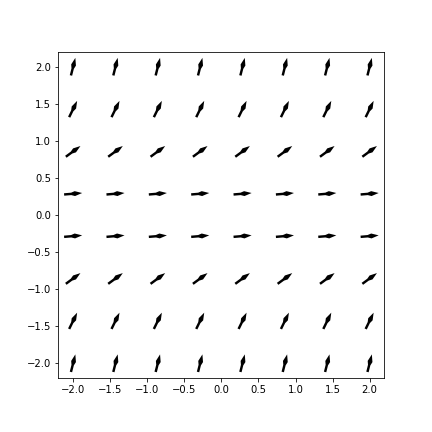
\includegraphics[width=0.4\textwidth]{../M2_IT/m2_it_ss_23_kurzaufgaben_richtungsfeld_3.png}} &
	\ifLoesung
	( {\textcolor{red}B} ) &
	\else
	( \quad ) &
	\fi
	\hspace*{-10mm} \raisebox{-0.8\height}{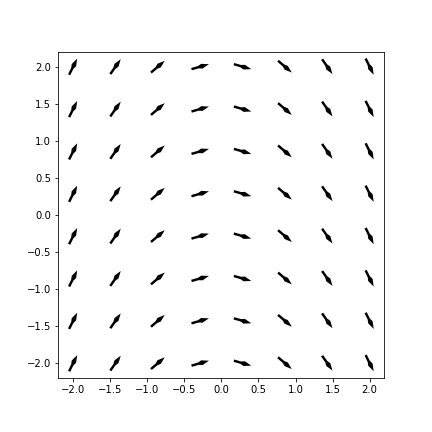
\includegraphics[width=0.4\textwidth]{../M2_IT/m2_it_ss_23_kurzaufgaben_richtungsfeld_2.png}}  \\
	\ifLoesung
	( {\textcolor{red}D} ) &
	\else
	( \quad ) &
	\fi
	\hspace*{-10mm} \raisebox{-0.8\height}{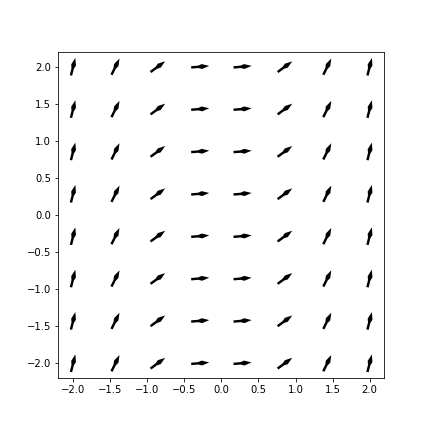
\includegraphics[width=0.4\textwidth]{../M2_IT/m2_it_ss_23_kurzaufgaben_richtungsfeld_4.png}} &
	\ifLoesung
	( {\textcolor{red}A} ) &
	\else
	( \quad ) &
	\fi
	\hspace*{-10mm} \raisebox{-0.8\height}{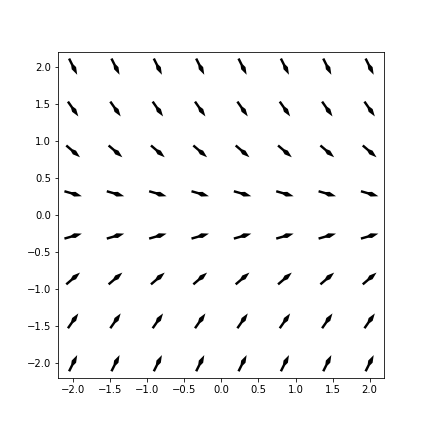
\includegraphics[width=0.4\textwidth]{../M2_IT/m2_it_ss_23_kurzaufgaben_richtungsfeld_1.png}}  \\
\end{tabular}

\ifLoesung
\mbox{}\hfill\Punkte{2 P}\\
\fi	

\pagebreak

	\item
		Welche Differenzialgleichung ist linear? Bitte kreuzen Sie den entsprechenden Eintrag an:

\ifLoesung 
\begin{tabular}{p{0.3\textwidth}p{0.2\textwidth}p{0.2\textwidth}}
	$y'' + 2 \, y' + y = \sin(x)$     & {\textcolor{red}X} linear &            $\square$ nicht linear\\
	$y'' + 2 \, y' + \sin(y) = 0$    & $\square$ linear  & {\textcolor{red}X} nicht linear\\
	$y'' + 2 \, y' + \sin(x) = 0$ &  {\textcolor{red}X} linear &            $\square$ nicht linear\\
	$y'' + 2 \, y' + \sin(x) \, y = 0$     & {\textcolor{red}X} linear &            $\square$ nicht linear\\
\end{tabular}
\hfill\Punkte{2 P}
\else
\begin{tabular}{p{0.3\textwidth}p{0.2\textwidth}p{0.2\textwidth}}
	$y'' + 2 \, y' + y = \sin(x)$     & $\square$ linear & $\square$ nicht linear\\
	$y'' + 2 \, y' + \sin(y) = 0$        & $\square$ linear & $\square$ nicht linear\\
	$y'' + 2 \, y' + \sin(x) = 0$     & $\square$ linear & $\square$ nicht linear\\
	$y'' + 2 \, y' + \sin(x) \, y = 0$ & $\square$ linear & $\square$ nicht linear\\
\end{tabular}
\fi

	\item
	Die Differenzialgleichung der Balkendurchbiegung $w(x)$ lautet:
	\[
		\frac{w''(x)}{({1 + (w'(x))^2})^{3/2}} = -\frac{M_y(x)}{E \, I_y} \, .
	\]
	Dabei bezeichnet $M_y(x)$ das Biegemoment an der Stelle $x$, $E$ das Elastizitätsmodul des Balkenmaterials und $I_y$ das axiale Flächenträgheitsmoment des Balkenquerschnitts.
	Stellen Sie die Differenzialgleichung mit Zustandsvariablen durch ein äquivalentes System von Differenzialgleichungen erster Ordnung dar.

\Loesung{}{
	Zwei Zustandsvariablen:
	\hfill\Punkte{2 P}
	\[
	z_1 = w(x), \, z_2 = w'(x) \, .
	\]
	System von Differenzialgleichungen erster Ordnung:
	\[
	\begin{array}{ccl}
		z'_1 & = & z_2 \, , \\
		z'_2 & = &  -\frac{M_y(x)}{E \, I_y} ({1 + z_2^2})^{3/2} \, .
	\end{array}
	\]
}
	
\pagebreak

	\item
		Folgende Frage wurde ChatGPT in der Version vom 12. Mai 2023 gestellt: 
		
		\begin{verbatim}
		Ein Teich enthält 1000 Liter Wasser. Täglich verdunsten 2% des Wassers im Teich und
		10 Liter Wasser werden nachgefüllt. Wieviel Wasser enthält der Teich nach 2 Tagen?
		\end{verbatim}
		
		Die Antwort lautete:
		
		\begin{verbatim}
		Zuerst berechnen wir die tägliche Verdunstungsmenge: 2% von 1000 Litern sind 20
		Liter. Da täglich 10 Liter Wasser nachgefüllt werden, verringert sich die Wasser-
		standsmenge um 10 Liter - 20 Liter = -10 Liter pro Tag. Nach 2 Tagen würde sich die
		Wassermenge im Teich um -10 Liter * 2 Tage = -20 Liter verringern. Da der Wasser-
		verlust die Nachfüllung übersteigt, enthält der Teich nach 2 Tagen kein Wasser mehr.
		\end{verbatim}
		
		Bestimmen Sie die korrekte Wassermenge im Teich nach $2$ Tagen mithilfe einer Differenzengleichung.
		
		\Loesung{5cm}{
			Differenzengleichung:
			\hfill\Punkte{2 P}
			\[
				T_{k+1} = 0.98 \, T_k + 10, \quad T_0 = 1000
			\]
			Nach einem Tag:
			\[
				T_1 = 0.98 \cdot 1000 + 10 = 990 
			\]
			Nach zwei Tagen:
			\[
				T_2 = 0.98 \cdot 990 + 10 =  980.2
			\]
			}
		
		\item
		Welchen Grenzwert $S$ hat die Reihe
		\[
			S = \sum_{k=2}^\infty \left(\frac{1}{3}\right)^k \, ?
		\]
		\Loesung{}{
			Geometrische Reihe mit $q = \frac{1}{3}$:
			\hfill\Punkte{2 P}
			\[
			\sum_{k=0}^\infty \left(\frac{1}{3}\right)^k  = \frac{1}{1 - q} = \frac{1}{1 - \frac{1}{3}} = \frac{3}{2} \, .
			\]
			Erste beiden Glieder:
			\[
				S = \sum_{k=2}^\infty \left(\frac{1}{3}\right)^k  = \sum_{k=0}^\infty \left(\frac{1}{3}\right)^k  - \left( 1 + \frac{1}{3} \right)  =   \frac{1}{6} 
			\]
		}
	\end{enumerate}

\end{Aufgabe}

\newpage

\endinput
\begin{Aufgabe}[8]% Vgl. SS 06
Gegeben ist das Anfangswertproblem 
\[
	y' = (y + 1) \, \cos(x), \quad  y(0) = 1.
\]
\begin{enumerate}
	\item
		Ist die Differenzialgleichung linear?
	\item
		Berechnen Sie die Lösung des Anfangswertproblems.   
	\item
		Ermitteln Sie einen Näherungswert $\tilde{y}_1$ für die Lösung des Anfangswertproblems an der Stelle $x=0.1$, indem Sie einen Schritt mit dem Euler-Polygonzugverfahren mit der Schrittweite $h = 0.1$ durchführen.
		Wie weit weicht der Näherungswert $\tilde{y}_1$ von der exakten Lösung ab? 
\end{enumerate}

\Loesung{}{
	\begin{enumerate}
		\item
			Linear.
			\hfill \Punkte{1 P}
		\item
			Trennung der Variablen:
			\hfill \Punkte{1 P}
			\[
				y' = (y + 1) \, \cos(x)
				\quad \Longrightarrow \quad 
				\int \frac{1}{y + 1} \, \mathrm{d}y = \int \cos(x) \, \mathrm{d}x
			\]
			Stammfunktionen:
			\hfill \Punkte{1 P}
			\[
				\ln\left(\left| y + 1 \right|\right) = \sin(x) + C_1, \quad C_1 \in \mathbb{R}
			\]
			Nach $y$ auflösen:
			\hfill \Punkte{1 P}
			\[
				\left| y + 1 \right| = \e^{ \sin(x) + C_1}
				\quad \Longrightarrow \quad 
				y + 1 = \pm \, \e^{C_1} \, \e^{ \sin(x)}
				\quad \Longrightarrow \quad
				y = C_2 \, \e^{ \sin(x)} - 1, \quad C_2 \in \mathbb{R}
			\]
		Anfangswert: 
		\hfill \Punkte{1 P}
		\[
		y(0) = C_2 - 1
		\quad \Longrightarrow \quad
		1 = C_2 - 1
		\quad \Longrightarrow \quad
		C_2 = 2
		\quad \Longrightarrow \quad
		y(x) =  2 \, \e^{ \sin(x)} - 1
		\]
		\item
		Euler-Polygonzugverfahren: 
		\hfill \Punkte{1 P}
		\[
		\tilde{y}_{n+1} = \tilde{y}_n + h \, ( \tilde{y}_n + 1) \, \cos(x_n),
		\]
		Schritt von $x_0=0$ nach $x_1=0.1$ mit Schrittweite $h=0.1$:
		\hfill \Punkte{1 P}
		\[
		\tilde{y}_1 = 1 + 0.1 \cdot (1 + 1) \, \cos(0)  = 1.2
		\]
		Abweichung:
		\hfill \Punkte{1 P}
		\[
		y(1.1) - \tilde{y}_1 = 2 \, \e^{ \sin(0.1)} - 1 - 1.2 \approx 0.009974
		\]	
	\end{enumerate}
}

\ifLoesung
\else
\newpage
\Loesung{}{}
\fi

\end{Aufgabe}

\newpage

\endinput
\begin{Aufgabe}[10]
Bestimmen Sie die allgemeine reelle Lösung der Differenzialgleichung
\[
	y'' + 4 \, y = 3 \, \cos( 2 \, x ) \, .
\]
\end{Aufgabe}

\Loesung{}{
	Charakteristische Gleichung:
	\hfill \Punkte{2 P} 
	\[
		\lambda^2 + 4 \, = 0
		\quad \Longrightarrow \quad
		\lambda_{1,2} = \pm 2 \, \mbox{i} 
	\]
	Homogene Lösung:
	\hfill \Punkte{1 P} 
	\[
		y_h(x) = C_1 \cos( 2 \, x )+ C_2 \sin( 2 \, x )
	\]
	Resonanzansatz für partikuläre Lösung:
	\hfill \Punkte{2 P} 
	\[
		y_p(x) = x \left( A \cos( 2 \, x )+ B \sin( 2 \, x ) \right)
	\]
	Erste Ableitung:
	\hfill \Punkte{1 P} 
	\[
		y'_p(x) = A \cos( 2 \, x )+ B \sin( 2 \, x ) + x \left( -2 \, A \sin( 2 \, x )+ 2 \, B \cos( 2 \, x ) \right)
	\]
	Zweite Ableitung:
	\hfill \Punkte{1 P} 
	\[
		y''_p(x) = -2 \, A \sin( 2 \, x )+ 2 \, B \cos( 2 \, x ) -2 \, A \sin( 2 \, x )+ 2 \, B \cos( 2 \, x ) 
		+ x \left( -4 \, A \cos( 2 \, x ) - 4 \, B \sin( 2 \, x ) \right)
	\]
	In Differenzialgleichung einsetzen:
	\hfill \Punkte{1 P} 
	\[
		\underbrace{-4 \, A \sin( 2 \, x )+ 4 \, B \cos( 2 \, x ) - 4\,  x \left( A \cos( 2 \, x ) + B \sin( 2 \, x ) \right)}_{\displaystyle y_p''}
		+ 4 \, 	\underbrace{x \left( A \cos( 2 \, x )+ B \sin( 2 \, x ) \right)}_{\displaystyle y_p} = 3 \, \cos( 2 \, x )
	\]
	$A$ und $B$ berechnen:
	\hfill \Punkte{1 P} 
	\[
		A = 0, \quad B = \frac{3}{4}
	\]
	Allgemeine reelle Lösung:
	\hfill \Punkte{1 P}
	\[
		y(x) = y_h(x) + y_p(x) = C_1 \cos( 2 \, x )+ C_2 \sin( 2 \, x ) +  \frac{3}{4} \, x \, \sin( 2 \, x )
	\]
}

\pagebreak

\ifLoesung
\else
\Loesung{}{}
\fi

\endinput
\begin{Aufgabe}[8] % vgl. SS 16, gleiche Matrix als DGL-System
	Gegeben ist das Differenzengleichungssystem
	\[
	\begin{array}{rcrcr}
		x_{k+1} & = & -2 \, x_k & + & 3 \, y_k,\\[1ex]
		y_{k+1} & = &	2 \, x_k & + & 3 \, y_k,\\
	\end{array}
	\quad k = 0,1,2,\ldots
	\]
	\begin{enumerate}
		\item
			Berechnen Sie die allgemeine Lösung des Differenzengleichungssystems.
		\item
			Ist das Differenzengleichungssystem asymptotisch stabil?
	\end{enumerate}
	
	\Loesung{}{
		\begin{enumerate}
			\item
			Vektor-Matrix-Form:
			\[
			\left(
			\begin{array}{l}
				x_{k+1}\\[1ex]
				y_{k+1}\\
			\end{array}
			\right)
			=
			\left(
			\begin{array}{rr}
				-2 & 3\\[1ex]
				  2 & 3\\
			\end{array}
			\right)
			\left(
			\begin{array}{l}
				x_{k}\\[1ex]
				y_{k}\\
			\end{array}
			\right)
			\hfill \Punkte{1 P} 
			\]
			Charakteristische Gleichung und Eigenwerte:
			\[
			\left|
			\begin{array}{cc}
				-2 - \lambda &                   3\\[1ex]
				                   2 & 3 - \lambda \\
			\end{array}
			\right|
			= \lambda^2 - \lambda - 12 = 0
			\quad \Longrightarrow \quad
			\lambda_1 = 4, \, \lambda_2 = -3 
			\hfill \Punkte{3 P} 
			\]		
			Eigenvektor für $\lambda_1 = 4$:
			\[
			\left(
			\begin{array}{rr}
				-6 &  3 \\[1ex]
				  2 & -1 \\
			\end{array}
			\right)
			\, \mathbf{v} = \mathbf{0}
			\quad \Longrightarrow \quad
			\mathbf{v} =
			\left(
			\begin{array}{r}
				\hphantom{-}1\\
				2\\
			\end{array}
			\right)  
			\hfill \Punkte{1 P} 
			\]  
			Eigenvektor für $\lambda_2 = -3$:
			\[
			\left(
			\begin{array}{rr}
				\hphantom{-}1 & \hphantom{-}3\\[1ex]
				2 & 6\\
			\end{array}
			\right)
			\, \mathbf{v} = \mathbf{0}
			\quad \Longrightarrow \quad
			\mathbf{v} =
			\left(
			\begin{array}{r}
				 3\\
				-1\\
			\end{array}
			\right)  
			\hfill \Punkte{1 P} 
			\]
			Allgemeine Lösung
			\[
			\left(
			\begin{array}{l}
				x_{k}\\
				y_{k}\\
			\end{array}
			\right)
			=
			C_1 \, 4^k
			\left(
			\begin{array}{r}
				\hphantom{-}1\\
									2\\
			\end{array}
			\right)   
			+ C_2 \, \left( -3 \right)^k
			\left(
			\begin{array}{r}
				3\\
				-1\\
			\end{array}
			\right)   
			\hfill \Punkte{1 P} 
			\]
			\item
			Die Beträge der Eigenwerte sind nicht kleiner als $1$.
			Somit ist das Differenzengleichungssystem nicht asymptotisch stabil.
			\hfill \Punkte{1 P} 
		\end{enumerate}
	}
	
	\ifLoesung
	\else
	\newpage
	\Loesung{}{}
	\fi
	
\end{Aufgabe} 

\newpage

\endinput
\begin{Aufgabe}[6] 
	Frau R. wird in 10 Jahren in Rente gehen und denkt über verschiedene Möglichkeiten des Geldanlegens nach, um ihre Rente aufzubessern. In den folgenden Aufgaben wird von einem jährlichen Zinssatz von 3\% ausgegangen.
	\begin{enumerate}
		\item Frau R. denkt zunächst daran, heute genügend Geld anzulegen, um mit Rentenbeginn bis zu 30 Jahre lang (also 30 mal) jeweils zu Beginn des Rentenjahres 6000 Euro abheben zu können. Welche Summe müsste Frau R. dafür heute mindestens anlegen?
		\item Frau R. fällt auf, dass sie die Inflationsrate einbeziehen sollte - sie geht von jährlich 3\% aus. Sie plant also mit ihrem Renteneintritt in zehn Jahren 6000 Euro und zu Beginn jedes weiteren Rentenjahres 3\% mehr als im Vorjahr abheben zu können - wieder bis zu 30 Jahre lang.
		\begin{itemize}
			\item Welche Summe plant Frau R. zu Beginn ihres 2., 5. bzw. 30. Rentenjahres abheben zu können?
			\item Welche Summe müsste zum Renteneintritt in 10 Jahren angespart sein, damit 30 Jahre lang wie beschrieben jeweils zu Beginn des Rentenjahres Geld abgehoben werden kann?
			\item Welche Summe müsste heute angelegt werden?
		\end{itemize}
	
	\end{enumerate}
	





\Loesung{}{
	\begin{enumerate}[label={\alph*)}]
		\item Der Endwert nach 30 Jahren Rente liegt bei \hfill\Punkte{3}
		\[R_{30}=E\cdot q\cdot\frac{q^{30}-1}{q-1}=6000\cdot 1.03\cdot\frac{1.03^{30}-1}{0.03}\approx 294016.07 \quad \text{(Euro)}\]
		Dieser Wert muss um 40 Jahre zurückdiskontiert werden und man erhält
		\[K_0=\frac{294016.07}{1.03^{40}}\approx90132.64 \quad \text{(Euro)}\]
		Hierbei wurde aufgerundet!
		\item Für das 2., 5. bzw. 30 Rentenjahr sind folgende Abhebungen geplant: \hfill\Punkte{1}
		\[6000\cdot 1.03=6180, \qquad 6000\cdot 1.03^{4}\approx 6753.05,\qquad 6000\cdot 1.03^{29}\approx 14139.39 \quad \text{(Euro)}\]
		Die angesparte Summe zum Renteneintritt muss bei \hfill\Punkte{1}
		\[6000+\frac{6000\cdot 1.03}{1.03}+\frac{6000\cdot 1.03^2}{1.03^2}+...+\frac{6000\cdot 1.03^{29}}{1.03^{29}}=30\cdot 6000=180000 \]
		Euro liegen. \\
		Diese Summe um 10 Jahre zurückdiskontiert, erhält man die Summe, die heute anzulegen ist. \hfill\Punkte{1}
		\[K_0=\frac{180000}{1.03^{10}}\approx 133936.91 \quad \text{(Euro)}\]
		Hier wurde wieder aufgerundet!
	\end{enumerate}
}

	\ifLoesung
\else
\newpage
\Loesung{}{}
\fi

\end{Aufgabe}

\newpage

\endinput
\begin{Aufgabe}[3] 
Ehepaar Schmidt hat vor 5 Jahren 10.000 Euro für seine Tochter Lina angelegt, in der Hoffnung 20 Jahre später (also in 15 Jahren) 20.000 Euro angespart zu haben. In den ersten Jahren gab es zweimal 1\%, zweimal 2\% und einmal 3\% Zinsen pro Jahr.
\begin{enumerate}
	\item Bestimmen Sie den effektiven Jahreszins für die ersten 5 Jahre (auf 1 Nachkommastelle gerundet).
	\item Angenommen der Zinssatz p für die kommenden 15 Jahre ist fest. Welchen Wert muss p (mindestens) haben, damit 20 Jahre nach Anlegen der 10.000 Euro tatsächlich (mindestens) 20.000 Euro angespart sind? Runden Sie auf 2 Nachkommastellen.
\end{enumerate}
	
\end{Aufgabe}

\Loesung{}{
\begin{enumerate}[label={\alph*)}] 
	\item \[p^*=100\cdot(\sqrt[5]{1.01^2\cdot 1.02^2\cdot 1.03}-1)\approx1.8\] \hfill\Punkte{1}
	\item Es gilt \hfill\Punkte{2}
	\[10000\cdot 1.01^2\cdot 1.02^2\cdot 1.03\cdot (1+\frac{p}{100})^{15}=20000\]
	Umstellen nach p ergibt
	\[p\approx 4.11\]
\end{enumerate}
}

\newpage

\endinput
\begin{Aufgabe}[9]

Gegeben ist das lineare Optimierungsproblem 
\[ 
 f(\vec x)=\vec c\cdot \vec x\stackrel{!}{=}\mathrm{Max}, \quad \mathbf A\vec x\leq \vec b,\quad \vec x\geq 0, 
\] 
mit 
\[ 
	\vec    c = \left(\begin{array}{c}  2\\ 1 \end{array}\right),\quad 
	\mathbf A = \left(\begin{array}{cc} -1 & 1\\ 0 & 1\\ 1 & 0 \end{array}\right),\quad 
	\vec    b = \left(\begin{array}{c}  0\\ 2\\ 4 \end{array}\right)\,. 
\] 

\begin{enumerate}
\item 	Zeichnen Sie den zulässigen Bereich in das gegebene Koordinatensystem ein.
\item 	Zeichnen Sie im zulässigen Bereich alle Punkte $(x_1,x_2)$ mit 
		$f(x_1,x_2)=6$ ein. 
\item 	Wenden Sie den Primalen Simplex-Algorithmus auf das lineare Optimierungsproblem an.
%\item	Wäre das gegebene Optimierungsproblem für 
%		$\vec c=\left(\begin{array}{c} 1\\ 1 \end{array}\right)$ lösbar? 
%		Begründen Sie Ihre Antwort. 
%\item 	Wäre das gegebene Optimierungsproblem für 
%		$\vec b=\left(\begin{array}{c} -6\\ 2 \\ 2 \end{array}\right)$ lösbar? 
%		Begründen Sie Ihre Antwort. \\
\end{enumerate}

\begin{center} 
\begin{tikzpicture}[xscale=1,yscale=1] 
 \draw[help lines,step=0.5] (-5.5,-1.0) grid (12.0,8.0); 
 \draw[->, darkgray, line width=1pt] (-1.0,0) -- (8.0,0) node[below] {$x_1$}; 
 \draw[->, darkgray, line width=1pt] (0,-1.0) -- (0,7) node[left] {$x_2$}; 
 %\foreach \i in {-1,...,-1} { \draw (\i,0.1) -- (\i,-0.1) node[below] {$\i$}; } 
 \foreach \i in {1,...,7} { \draw (\i,0.1) -- (\i,-0.1) node[below] {$\i$}; } 
 \foreach \i in {1,...,6} { \draw (0.1,\i) -- (-0.1,\i) node[left] {$\i$}; } 
 %\foreach \i in {-1,...,-1} {\draw (0.1,\i) -- (-0.1,\i) node[left] {$\i$};} 
 \ifLoesung 
	%\coordinate[] (P) at (0,3); \fill (P) circle (2pt); 
	\coordinate[label=] (Q) at (4,0); \fill (Q) circle (2pt); 
	\coordinate[label=] (R) at (0,0); \fill (R) circle (2pt); 
	\coordinate[label= ] (S) at (2,2); \fill (S) circle (2pt); 
	\coordinate[label= ] (T) at (4,2); \fill (T) circle (2pt); 
	\coordinate[label= right: Zulässigkeitsbereich  ] (S1) at (0.5,0.5);  
	\coordinate[label= right: Isolinie ] (S2) at (1.75,1.5); 

	\draw[ultra thick,-] (0,0)--(2,2); 
	\draw[ultra thick,-] (2,2)--(4,2); 
	\draw[ultra thick,-] (4,2)--(4,0);
	\draw[ultra thick,-] (0,0)--(4,0); 
	%\draw[ultra thick,-] (0,0)--(0,3); 
	\draw[gray, dashed, ultra thick,-] (2,2)--(3,0); 
\fi
 \end{tikzpicture} 
\end{center} 

\newpage


\Loesung{}{

% ----------------------------------------------------------------------------
% MATLAB-Quelltext
% p  = 5;
% K0 = 30000;
% N1 = -K0 + 15000/(1+p/100) + 17000/(1+p/100)^2
% N2 = -K0 + 16500/(1+p/100) + 16000/(1+p/100)^2
% K2 = K0*(1+5/(12*100))^(12*2)
% pstern= 100*((1+p/(12*100))^12-1)
% ----------------------------------------------------------------------------

\begin{enumerate}
\item Zulässigkeitsbereich: siehe Skizze. 				
	\hfill\Punkte{2} 

\item Isolinie $f(x_1,x_2)=6$: siehe Skizze.			
	\hfill\Punkte{1}

\item 
	Das LOP ist in Standardformat gegeben und wegen $\vec 0 \leq \vec b$ ist $\vec 0$ ein Eckpunkt des zulässigen Bereichs. \\ 
	Das Ausgangstableau lautet 
	\[ 
	\begin{array}{c|cc|ccc|c} 
	\mbox{BV} &  x_1                   & x_2                    & z_1                    & z_2                    & z_3                    & b_i  \\ \hline 
	z_1      & -1 & 1 & 1 & 0 & 0 & 0  \\ 
	z_2      & 0 & 1 & 0 & 1 & 0 & 2 \\ 
	z_3      & 1 & 0 & 0 & 0 & 1 & 4 \\ \hline 
	f        & 2 & 1 & 0 & 0 & 0 & 0 \\ 
	\end{array} 
	\hfill\Punkte{1}
	\] 
$1$. Schritt: 
	Pivot-Spalte: $1$; Pivot-Zeile: $3$. Die Nichbasisvariable $x_{1}$ wird in die Basis aufgenommen. Dies führt auf das Tableau 
	\[ 
	\begin{array}{c|cc|ccc|c} 
	\mbox{BV}   &  x_1                    & x_2                     & z_1                     & z_2                     & z_3                     & b_i  \\ \hline 
	z_1 & 0 & 1 & 1 & 0 & 1 & 4\\ 
	z_2 & 0 & 1 & 0 & 1 & 0 & 2\\ 
	x_{1}  & 1 & 0 & 0 & 0 & 1 & 4\\ \hline 
	f          & 0 & 1 & 0 & 0 & -2 & -8\\ 
	\end{array} 
	\hfill\Punkte{2}
	\] 
$2$. Schritt: 
	Pivot-Spalte: $2$; Pivot-Zeile: $2$. 
	Die Nichbasisvariable $x_{2}$ wird in die Basis aufgenommen. Dies führt auf das Tableau 
	\[ 
	\begin{array}{c|cc|ccc|c} 
	\mbox{BV}   &  x_1                    & x_2                     & z_1                     & z_2                     & z_3                     & b_i  \\ \hline 
	z_{1}  & 0 & 0 & 1 & -1 & 1 & 2\\ 
	x_2 & 0 & 1 & 0 & 1 & 0 & 2\\ 
	x_{1}  & 1 & 0 & 0 & 0 & 1 & 4\\ \hline 
	f          & 0 & 0 & 0 & -1 & -2 & -10\\ 
	\end{array} 
	\hfill\Punkte{2}
	\] 
Die Zielfunktionszeile enthält nur Elemente $\leq 0$. Dies entspricht der 1. Abbruchbedingung. \\ 
Die optimale zulässige Lösung ist $(x_1,x_2)=(4,2)$ mit $f(x_1,x_2)= 10$. 
%Bemerkung: Falls die letzte Zeile bei Gau\ss-Operationen skaliert wurde, muss diese Skalierung am Ende r\"uckg\"angig gemacht werden, damit der Wert in der Ecke unten rechts stimmt. 
\hfill\Punkte{1}
\end{enumerate}

}

\ifLoesung
\else
\newpage
\Loesung{}{}
\fi

\end{Aufgabe}

\newpage

\endinput
\end{document}
